\documentclass[12pt]{article}
\usepackage[spanish,es-tabla]{babel}
\usepackage[square,numbers]{natbib}
\usepackage{url}
\usepackage[utf8x]{inputenc}
\usepackage{amsmath}
\usepackage{graphicx}
\usepackage{parskip}
\usepackage{fancyhdr}
\usepackage{vmargin}
\usepackage[ddmmyy]{datetime}
\usepackage{anyfontsize}
\usepackage{xcolor}
\usepackage[nooldvoltagedirection]{circuitikz}
\usepackage[locale=FR]{siunitx}
\setmarginsrb{3 cm}{2.5 cm}{3 cm}{2.5 cm}{1 cm}{1.5 cm}{1 cm}{1.5 cm}
%Includes "References" in the table of contents
\usepackage[nottoc]{tocbibind}
%%%%%%%%%%%%%%%%%%%%%%%%%%%%%%%%%%%%%%%%%%%%%%%%%%%%%%%%%%%%%%%%%%%%%%%%%%%%%%%%%%%%%%%%%
% DATOS GENERALES
\title{Titulo del Trabajo}	    				% Titulo del trabajo.
\author{Nombre Apellido}					% Nombre y apellido
\newcommand{\padron}{123456}   				% Padrón
\newcommand{\tpnumber}{n}       				% Número de trabajo práctico
\newcommand{\codigo}{80.00}					% Código de la Materia
\newcommand{\materia}{Nombre de la Meteria}	% Nombre de la materia
\date{\today}								% Fecha (automática, no tocar)

\makeatletter
\let\thetitle\@title
\let\theauthor\@author
\let\thedate\@date
\makeatother
\pagestyle{fancy}
\fancyhf{}
\rhead{\theauthor}
\lhead{\thetitle}
\cfoot{\thepage}


\bibliographystyle{plainnat}

%%%%%%%%%%%%%%%%%%%%%%%%%%%%%%%%%%%%%%%%%%%%%%%%%%%%%%%%%%%%%%%%%%%%%%%%%%%%%%%%%%%%%%%%%
\begin{document}
%% CARATULA - INDIVIDUAL
\begin{titlepage}
    
\includegraphics[width = \linewidth]{img/logofiuba.png}\\[1.0 cm]	    % Logo fiuba
    \centering
	\textsc{\Large \codigo}\\[0.2 cm] 
	\textsc{\large \materia}\\[4 cm]
	\textcolor{cyan}{{\fontsize{40}{60}\selectfont \bfseries \thetitle}}\\[0.5cm]
	{ \Large \bfseries Trabajo Práctico N$^\circ$\tpnumber}\\[5cm]
	
	
    \noindent\makebox[\linewidth]{\rule{\textwidth}{0.4pt}}\\[0.5cm]
    \begin{minipage}{.4\textwidth}
    \textbf{Autor}:\\
    \theauthor
    \end{minipage}%
    \begin{minipage}{.4\textwidth}
    \textbf{Padrón}:\\
    \padron
    \end{minipage}%
    \begin{minipage}{.2\textwidth}
    \textbf{Fecha}:\\
    \thedate
    \end{minipage}
 
	\vfill
\end{titlepage}

%% CARATULA - GRUPAL
%\begin{titlepage}
%    
\includegraphics[scale = 0.71]{img/logofiuba.png}\\[1.0 cm]	    % Logo fiuba
%    \centering
%	\textsc{\Large \codigo}\\[0.2 cm] %Codigo de la materia
%	\textsc{\large \materia}\\[4 cm] %Nombre de la materia
%	\textcolor{cyan}{{\fontsize{40}{60}\selectfont \bfseries \thetitle}}\\[0.5cm]
%	{ \Large \bfseries Trabajo Práctico N$^\circ$\tpnumber}\\[5cm]
%  \begin{minipage}[t]{.5\textwidth}
%    \textbf{Autor}:\\
%    Estudiante 1\\
%    Estudiante 2\\
%    Estudiante 3\\
%    \end{minipage}%
%    \begin{minipage}[t]{.4\textwidth}
%    \textbf{Padrón}:\\
%    123456\\
%    123456\\
%    123456\\
%    \end{minipage}%
%    \begin{minipage}[t]{.2\textwidth}
%    \textbf{Fecha}:\\
%    \thedate
%    \end{minipage}
%	\vfill	
%\end{titlepage}

%%%%%%%%%%%%%%%%%%%%%%%%%%%%%%%%%%%%%%%%%%%%%%%%%%%%%%%%%%%%%%%%%%%%%%%%%%%%%%%%%%%%%%%%%

%\tableofcontents    % Comentar o descomentar segun se desee o no una pagina con el indice
%\pagebreak

%%%%%%%%%%%%%%%%%%%%%%%%%%%%%%%%%%%%%%%%%%%%%%%%%%%%%%%%%%%%%%%%%%%%%%%%%%%%%%%%%%%%%%%%%
\section{Introducción}

\section{Ejemplos}

\subsection{Circuitos}
\begin{figure}[!ht]
  \centering
  \begin{circuitikz}[american]
  \draw (2,4.0) to[R, l=$R_{3}$,*-] (2,2.0);
  \draw (2,2.0) to[R, l=$R_{4}$, -*] (2,-0.0);
  \draw (4,2.0) to[R, l=$R_{5}$] (4,-0.0);
  \draw (0,-0.0) to[short] (2,-0.0);
  \draw (2,-0.0) to[short] (4,-0.0);
  \draw (2,2.0) to[short, *-] (4,2.0);
  \draw (0,4.0) to[short] (2,4.0);
  \draw (0,4.0) to[battery2, l_=V] (0,-0.0);
  \draw (2,4.4) node[]{A};
  \draw (1.6,2.0) node[]{B};
  \draw (2,-0.4) node[]{C};
  \end{circuitikz}
  \caption{Circuito 1}
\end{figure}

\subsection{Insertar Imagen}

\begin{figure}[!ht]
  \centering  %figura centrada en el texto
  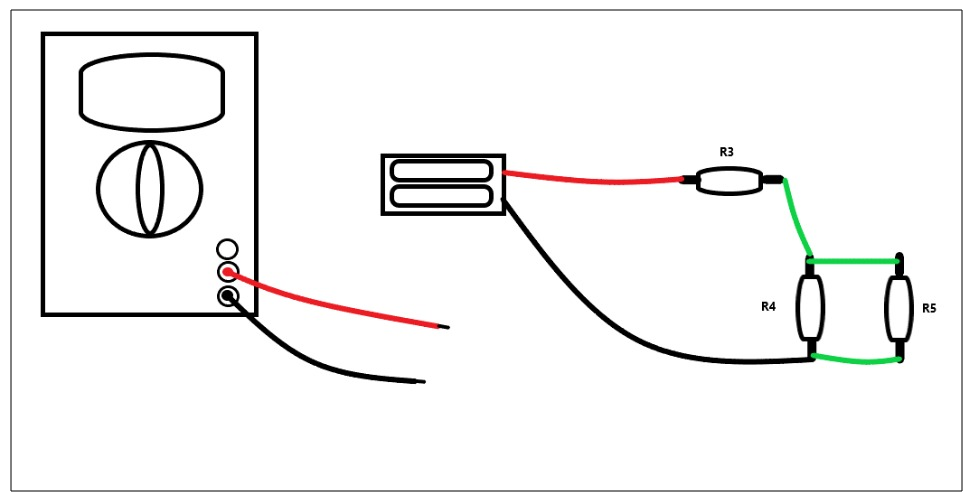
\includegraphics[width=0.9\linewidth]{img/banco_medicion.png}
  \caption{Banco de Medición}    %texto que acompaña a la imagen por debajo
  \label{fig:bancoMedicion}  %etiqueta para referenciar la figura
\end{figure}

\subsection{Tablas}

\begin{table}[!ht]
    \begin{center}
      \begin{tabular}{|c|c|c|} \hline 
        Escala:  \SI{200}{\volt} & Valor en pantalla & Incertidumbre\\ \hline 
        $V^{AB}$ & \SI{0.5}{\volt} & $\pm \SI{0.5}{\volt}$\\ \hline 
        $V^{BC}$ & \SI{2.5}{\volt} & $\pm \SI{0.5}{\volt}$\\ \hline 
        $V^{AC}$ & \SI{3.0}{\volt} & $\pm \SI{0.5}{\volt}$\\ \hline 
      \end{tabular}
      \caption{Mediciones de tensión en escala \SI{200}{\volt}}
    \end{center}
  \end{table}

\subsection{Ecuaciones}
Para insertar símbolos matemáticos en el texto, se encierra la expresión entre signos \$, como se muestra a continuación $\omega$, $\Omega$, $\alpha$, $\beta$. Noten que el símbolo de ohm se representa con la letra griega omega mayúscula $\Omega$. Así es más fácil usar subindices $R_1$ $R_{13}$ y superindices $x^2$ $x^{y+z}$.

Para insertar una ecuación, se puede hacer así

\begin{align}
    V_{12} = I R_1 + I R_2
\end{align}

Para varias ecuaciones:

\begin{align}
    V_{12} = I R_1 + I R_2\\
    V_{12} = 2A \cdot 3\Omega + 2A \cdot 5\Omega\\
    V_{12} = 16V
\end{align}

O asi, donde el símbolo \& se alinea para todas las ecuaciones, sin importar donde esté.

\begin{align}
    V_{12} & = I R_1 + I R_2\\
    V_{12} & = 2A \cdot 3\Omega + 2A \cdot 5\Omega\\
    V_{12} & = 16V
\end{align}

El comando ``cdot'' es conveniente para expresar multiplicación, dejando un espacio entre factores, para mejor entendimiento.
%%%%%%%%%%%%%%%%%%%%%%%%%%%%%%%%%%%%%%%%%%%%%%%%%%%%%%%%%%%%%%%%%%%%%%%%%%%%%%%%%%%%%%%%%%%%%%%%%%%%%%%%%%

\section{Conclusiones}


\pagebreak
% BIBLIOGRAFIA
\bibliography{bibliografia}
\nocite{*} % Muestra toda la bibliografia o solo la citada

\end{document}
